O diagrama da Figura 2 resume um sistema de gestão agrícola com classes para Usuário, Propriedade, Talhão e 
Diagnóstico, além de ServidorNode, ProcessamentoPython, BancoDeDados e PainelAdmin. Juntas, elas cobrem do 
login e cadastro ao registro de áreas, classificação de imagens por CNN e armazenamento/gestão dos resultados.

\medskip
\noindent{As principais classes e seus papéis são:}
\begin{itemize}[itemsep=0.6em, topsep=0.3em, parsep=0pt]
    \item \textbf{Propriedade}: Cadastra e gerencia propriedades rurais (endereço completo, cidade, CEP), vinculadas a um idUsuario; permite criar/editar e listar talhões da propriedade.
    \item \textbf{Usuario}: Mantém dados pessoais e de autenticação (nome, e-mail, telefone, senha, tipo); oferece cadastro, edição de perfil e login para controle de acesso.
    \item \textbf{Talhao}: Subárea da propriedade. Guarda id e nome, ligado a uma Propriedade. Permite cadastrar/editar e consultar o histórico de diagnósticos do local.
    \item \textbf{Diagnostico}: Registro de análise por imagem de folha. Liga-se a um Talhão e salva data, resultado e probabilidade. Métodos: enviar imagem, receber e visualizar resultado.
    \item \textbf{ServidorNode}: Faz a ponte do frontend com a API; recebe requisições, encaminha para o módulo Python, monitora status e salva resultados no banco.
    \item \textbf{ProcessamentoPython}: Executa classificação de imagens com CNN, controla versões dos modelos e permite atualizar/rodar modelos para análise agrícola.
    \item \textbf{BancoDeDados}: Gerencia a conexão e as operações CRUD; insere, consulta e atualiza registros, sustentando a persistência de todo o sistema.
    \item \textbf{PainelAdmin}: Área do administrador para gestão global; visualiza usuários, monitora o sistema e atualiza modelos de CNN, garantindo o controle da plataforma.
\end{itemize}

\begin{figure}[H]
\centering
\caption{Diagrama de classe}%
\label{fig:diagrama-classe}
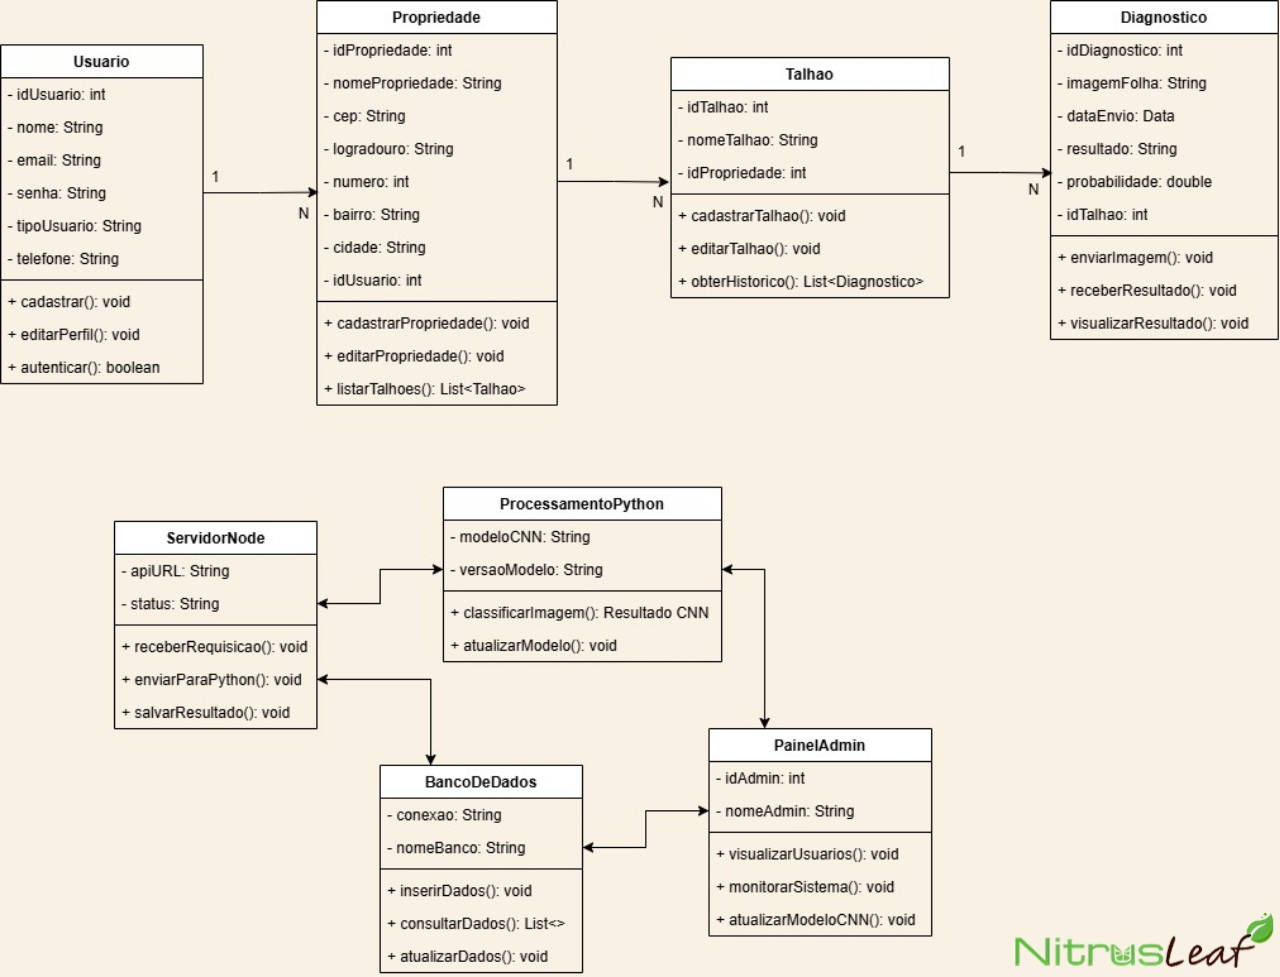
\includegraphics[width=0.8\textwidth]{Images/DiagramaDeClasses.jpg}
\SourceOrNote{Equipe 21 - Vitalliz (2025)}
\end{figure}

O diagrama mostra claramente os relacionamentos de composição e agregação
entre as entidades, com cardinalidades bem definidas. Além disso, os métodos estão
especificados em várias classes, indicando a lógica operacional do sistema, e a
estrutura geral está organizada para refletir um fluxo de uso coerente com os casos de
uso anteriores.
\medskip